\chap{Timer Interrupt and LED Scanning}

% \section{Introduction}
% Timers are one of the most important features in modern micro-controllers. They allow us to measure how long something takes to execute, create non-blocking code, precisely control pin timing, and even run operating systems. In this manual, how to configure a timer using STM32CubeIDE is presented how to use them to flash an LED. Finally, students are proposed to finalize 10 exercises using timer interrupt for applications based LED Scanning.

% \begin{figure}[!htp]
%     \centering
%     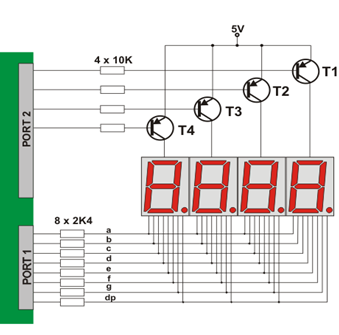
\includegraphics[width=3.5in]{source/picture/bai_2/led_scanning1.png}
%     \caption{\textit{Four seven segment LED interface for a micro-controller}}
%     \label{bai2_intro1}
% \end{figure}


% Design an interface for with multiple LED (seven segment or matrix) displays which is to be controlled is depends on the number of input and output pins needed for controlling all the LEDs in the given matrix display, the amount of current that each pin can source and sink and the speed at which the micro-controller can send out control signals. With all these specifications, interfacing can be done for 4 seven segment LEDs with a micro-controller is proposed in the figure above. \\


% In the above diagram each seven segment display is having 8 internal LEDs, leading to the total number of LEDs is 32. However, not all the LEDs are required to turn ON, but one of them is needed. Therefore, only 12 lines are needed to control the whole 4 seven segment LEDs.   By controlling with the micro-controller, we can turn ON an LED during a same interval \textbf{$T_S$}. Therfore, the period for controlling all 4 seven segment LEDs is \textbf{$4T_S$}. In other words, these LEDs are scanned at frequecy \textbf{$f = 1 / 4T_S$}. Finally, it is obviously that if the frequency is greater than 30Hz (e.g. f = 50Hz), it seems that all LEDs are turn ON at the same time.\\

% In this manual, the timer interrupt is used to design the interval $T_S$ for LED scanning. Unfortunately, the simulation on Proteus can not execute at high frequency, the frequency $f$ is set to a low value (e.g. 1Hz). In a real implementation, this frequency should be 50Hz.


% \newpage
% \section{Timer Interrupt Setup}
% \textbf{Step 1: } Create a simple project, which LED connected to PA5. The manual can be found in the first lab.\\

% \textbf{Step 2: } Check the clock source of the system on the tab \textbf{Clock Configuration} (from *.ioc file). In the default configuration, the internal clock source is used with 8MHz, as shown in the figure bellow.

% \begin{figure}[!htp]
%     \centering
%     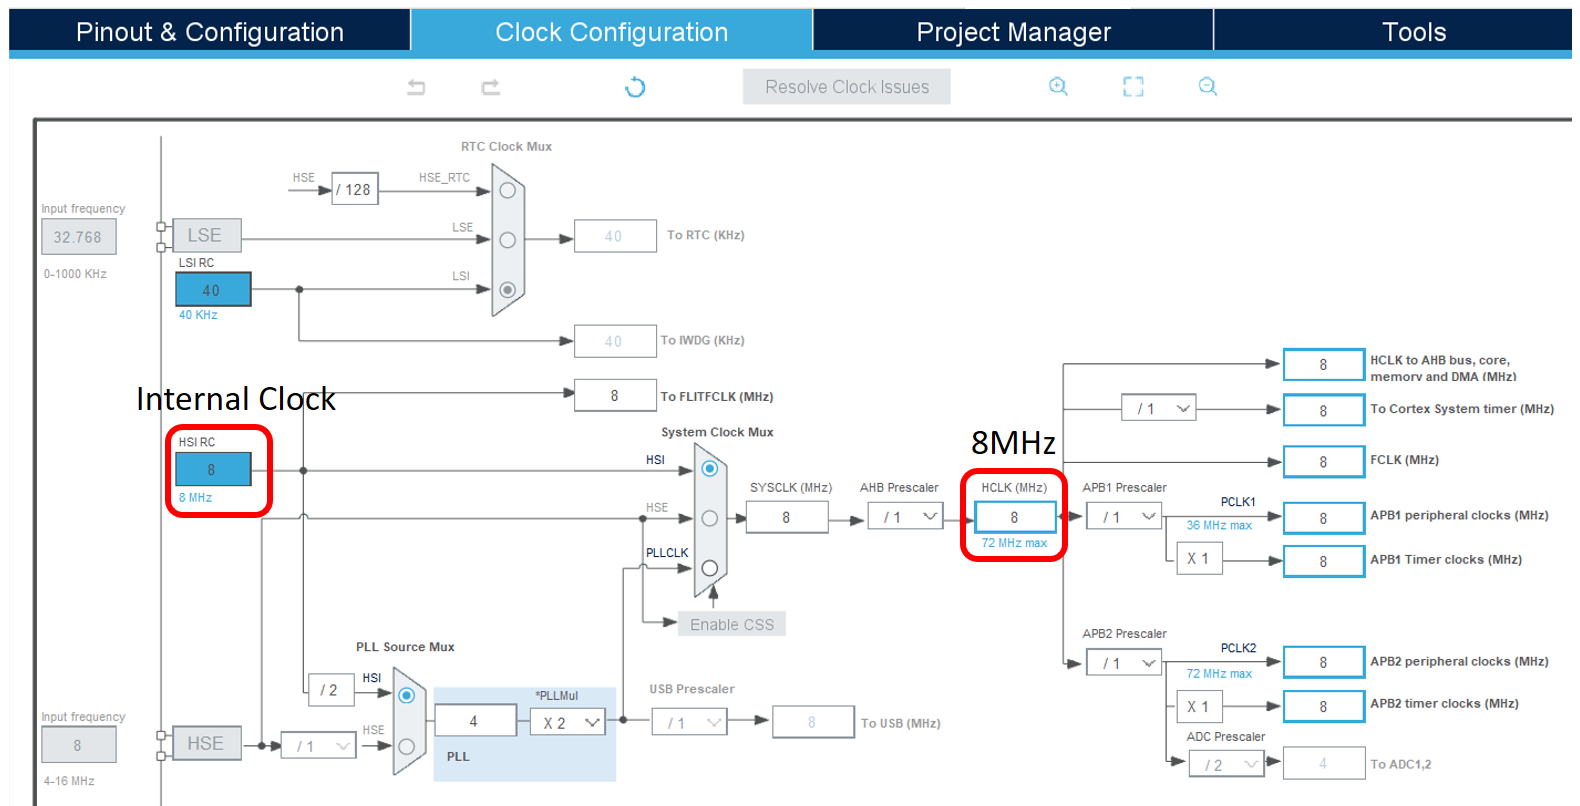
\includegraphics[width=5.5in]{source/picture/bai_2/lab2_m1.PNG}
%     \caption{\textit{Default clock source for the system}}
%     \label{bai2_m1}
% \end{figure}

% \textbf{Step 3: } Configure the timer on the \textbf{Parameter Settings}, as follows:
% \begin{figure}[!htp]
%     \centering
%     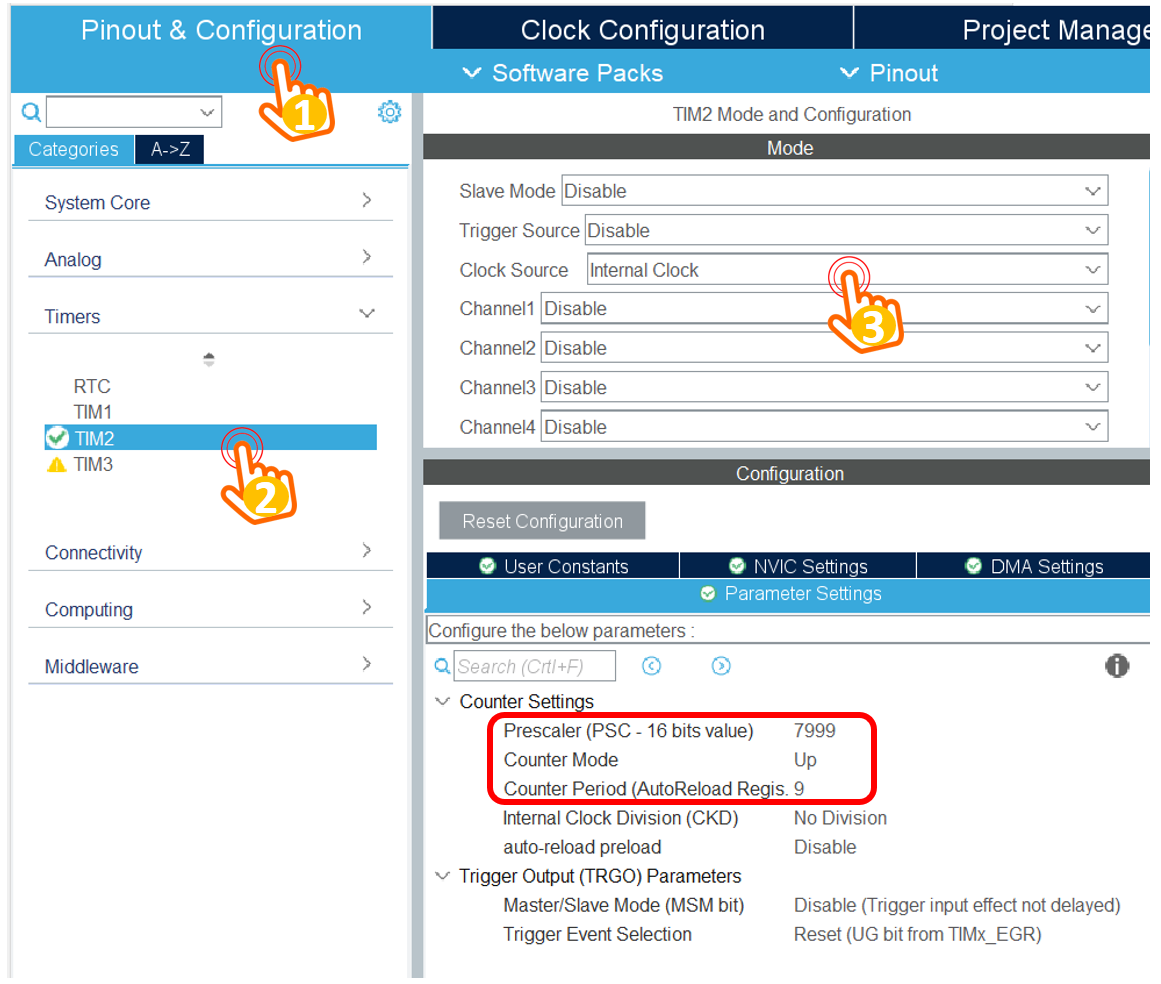
\includegraphics[width=3.5in]{source/picture/bai_2/lab2_m2.PNG}
%     \caption{\textit{Configure for Timer 2}}
%     \label{bai2_m2}
% \end{figure}

% Select the clock source for timer 2 to the \textbf{Internal Clock}. Finally, set the prescaller and the counter to 7999 and 9, respectively. These values are explained as follows:
% \begin{itemize}
%     \item The target is to set an interrupt timer to 10ms
%     \item The clock source is 8MHz, by setting the prescaller to 7999, the input clock source to the timer is \textbf{8MHz/(7999+1) = 1000Hz}.
%     \item The interrupt is raised when the timer counter is counted from 0 to 9, meaning that the frequency is divided by 10, which is 100Hz.
%     \item The frequency of the timer interrupt is 100Hz, meaning that the period is \textbf{1/100Hz = 10ms}.
% \end{itemize}

% \textbf{Step 4: } Enable the timer interrupt by switching to \textbf{NIVC Settings} tab, as follows:

% \begin{figure}[!htp]
%     \centering
%     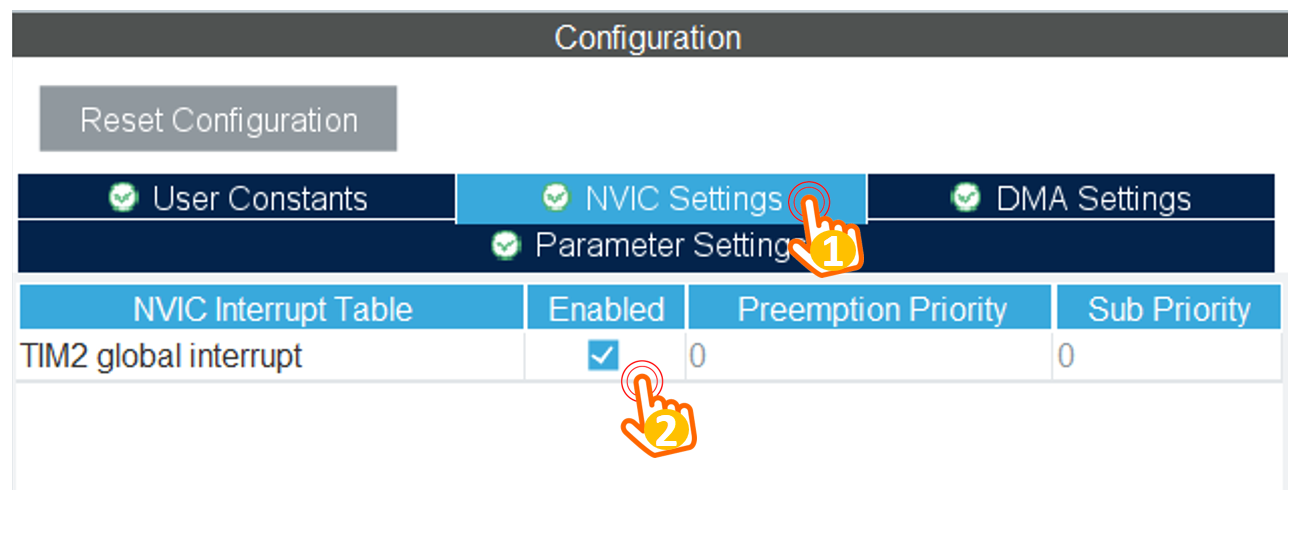
\includegraphics[width=4in]{source/picture/bai_2/lab2_m3.PNG}
%     \caption{\textit{Enable timer interrupt}}
%     \label{bai2_m3}
% \end{figure}

% Finally, save the configuration file to generate the source code.\\

% \textbf{Step 5: } On the \textbf{main()} function, call the timer init function, as follows:

% \begin{lstlisting}[caption=Init the timer interrupt in main]
% int main(void)
% {
%   HAL_Init();
%   SystemClock_Config();

%   MX_GPIO_Init();
%   MX_TIM2_Init();
  
%   /* USER CODE BEGIN 2 */
%   HAL_TIM_Base_Start_IT(&htim2);
%   /* USER CODE END 2 */g3

%   while (1){
  
%   }
% }
% \end{lstlisting}

% Please put the init function in a right place to avoid conflicts when code generation is executed (e.g. ioc file is updated).\\
% \newpage
% \textbf{Step 6: } Add the interrupt service routine function, this function is invoked every 10ms, as follows:

% \begin{lstlisting}[caption=Add an interrupt service routine]
% /* USER CODE BEGIN 4 */
% void HAL_TIM_PeriodElapsedCallback(TIM_HandleTypeDef *htim){
	
% }
% /* USER CODE END 4 */
% \end{lstlisting}

% \textbf{Step 7: } To run a LED Blinky demo using interrupt, a short manual is presented as follows:
% \begin{lstlisting}[caption=LED Blinky using timer interrupt]
% /* USER CODE BEGIN 4 */
% int counter = 100;
% void HAL_TIM_PeriodElapsedCallback(TIM_HandleTypeDef *htim){
% 	counter--;
% 	if(counter <= 0){
% 		counter = 100;
% 		HAL_GPIO_TogglePin(LED_RED_GPIO_Port, LED_RED_Pin);
% 	}
% }
% /* USER CODE END 4 */
% \end{lstlisting}

% The \textbf{HAL\_TIM\_PeriodElapsedCallback} function is an infinite loop, which is invoked every cycle of the timer 2, in this case, is 10ms.\\



\newpage
\section{Exercise and Report}
\subsection{Exercise 1}
% The first exercise show how to interface for multiple seven segment LEDs to STM32F103C6 micro-controller (MCU). Seven segment displays are common anode type, meaning that the anode of all LEDs are tied together as a single terminal and cathodes are left alone as individual pins. \\

% In order to save the resource of the MCU, individual cathode pins from all the seven segment LEDs are connected together, and connect to 7 pins of the MCU. These pins are popular known as the \textbf{signal pins}. Meanwhile, the anode pin of each seven segment LEDs are controlled under a power enabling circuit, for instance, an PNP transistor. At a given time, only one seven segment LED is turned on. However, if the delay is small enough, it seems that all LEDs are enabling. \\

% Implement the circuit simulation in Proteus with two 7-SEGMENT LEDs as following:

\begin{figure}[!htp]
    \centering
    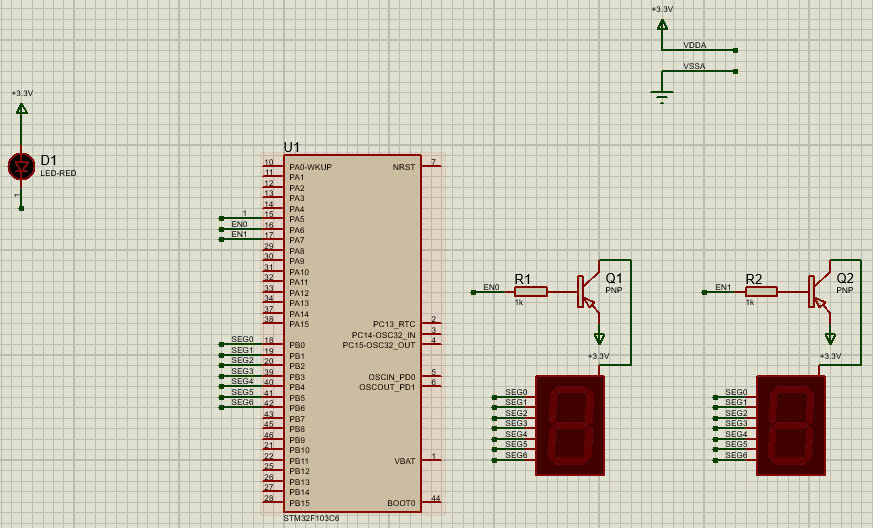
\includegraphics[width=5.5in]{source/picture/bai_2/pic1.jpg}
    \caption{\textit{ Schematic in Proteus}}
    \label{bai2_pic1a}
\end{figure}
\begin{lstlisting}[caption=main.c]
/* USER CODE BEGIN 2 */
  HAL_TIM_Base_Start_IT (& htim2 ) ;
  setTimer(0, 500);
  /* USER CODE END 2 */

  /* Infinite loop */
  /* USER CODE BEGIN WHILE */
  while (1)
  {
	  if(isTimerExpired(0)==1){
		  setTimer(0, 500);
		  Ex1_run();
	  }
    /* USER CODE END WHILE */

    /* USER CODE BEGIN 3 */
  }
\end{lstlisting}
\begin{lstlisting}[caption=software$\_$timer1.c]
#include "software_timer1.h"

#define MAX_COUNTER 10
#define TIMER_TICK 10

int timer_counter[MAX_COUNTER];
int timer_flag[MAX_COUNTER];
int index_led=0;

void display7SEG(int num) {
      const uint8_t segmentMap[10] = {
          0b11111100,
          0b01100000,
          0b11011010,
          0b11110010,
          0b01100110,
          0b10110110,
          0b10111110,
          0b11100000,
          0b11111110,
          0b11110110
      };
      HAL_GPIO_WritePin(SEG0_GPIO_Port, SEG0_Pin, (segmentMap[num] & 0b10000000) ? GPIO_PIN_RESET : GPIO_PIN_SET);
      HAL_GPIO_WritePin(SEG1_GPIO_Port, SEG1_Pin, (segmentMap[num] & 0b01000000) ? GPIO_PIN_RESET : GPIO_PIN_SET);
      HAL_GPIO_WritePin(SEG2_GPIO_Port, SEG2_Pin, (segmentMap[num] & 0b00100000) ? GPIO_PIN_RESET : GPIO_PIN_SET);
      HAL_GPIO_WritePin(SEG3_GPIO_Port, SEG3_Pin, (segmentMap[num] & 0b00010000) ? GPIO_PIN_RESET : GPIO_PIN_SET);
      HAL_GPIO_WritePin(SEG4_GPIO_Port, SEG4_Pin, (segmentMap[num] & 0b00001000) ? GPIO_PIN_RESET : GPIO_PIN_SET);
      HAL_GPIO_WritePin(SEG5_GPIO_Port, SEG5_Pin, (segmentMap[num] & 0b00000100) ? GPIO_PIN_RESET : GPIO_PIN_SET);
      HAL_GPIO_WritePin(SEG6_GPIO_Port, SEG6_Pin, (segmentMap[num] & 0b00000010) ? GPIO_PIN_RESET : GPIO_PIN_SET);
  }
  
void Ex1_run(){
	if(index_led>=2) index_led=0;
	index_led++;
	if(index_led<=1){
		HAL_GPIO_WritePin(EN1_GPIO_Port, EN1_Pin, SET);
		HAL_GPIO_WritePin(EN0_GPIO_Port, EN0_Pin, RESET);
		display7SEG(1);
	}
	if(index_led>=2){
		HAL_GPIO_WritePin(EN0_GPIO_Port, EN0_Pin, SET);
		HAL_GPIO_WritePin(EN1_GPIO_Port, EN1_Pin, RESET);
		display7SEG(2);
	}
}

void setTimer(int index, int value){
	timer_counter[index]=value/TIMER_TICK;
	timer_flag[index]=0;
}

int isTimerExpired(int index){
	if(timer_flag[index]==1){
		timer_flag[index]=0;
		return 1;
	}
	return 0;
}

void timerRun(){
	for(int i=0;i<MAX_COUNTER;i++){
		  if(timer_counter[i]>0){
			timer_counter[i]--;
			if(timer_counter[i]<=0) timer_flag[i]=1;
		}
    }
}
\end{lstlisting}
Short question: Tần số của quá trình quét là $\dfrac{1}{2\times0.5}$ = 1 Hz.
% Components used in the schematic are listed bellow:
% \begin{itemize}
%     \item 7SEG-COM-ANODE (connected from PB0 to PB6)
%     \item LED-RED
%     \item PNP
%     \item RES
%     \item STM32F103C6
% \end{itemize}


% Students are proposed to use the function \textbf{display7SEG(int num)} in the Lab 1 in this exercise. Implement the source code in the interrupt callback function to display number \textbf{"1"} on the first seven segment and number \textbf{"2"} for second one. The switching time between 2 LEDs is half of second. \\

% \textbf{Report 1: } Capture your schematic from Proteus and show in the report.\\

% \textbf{Report 2: } Present your source code in the \textbf{HAL\_TIM\_PeriodElapsedCallback} function.\\

% \textbf{Short question: } What is the frequency of the scanning process?\\
\newpage
\subsection{Exercise 2}
\begin{figure}[!htp]
    \centering
    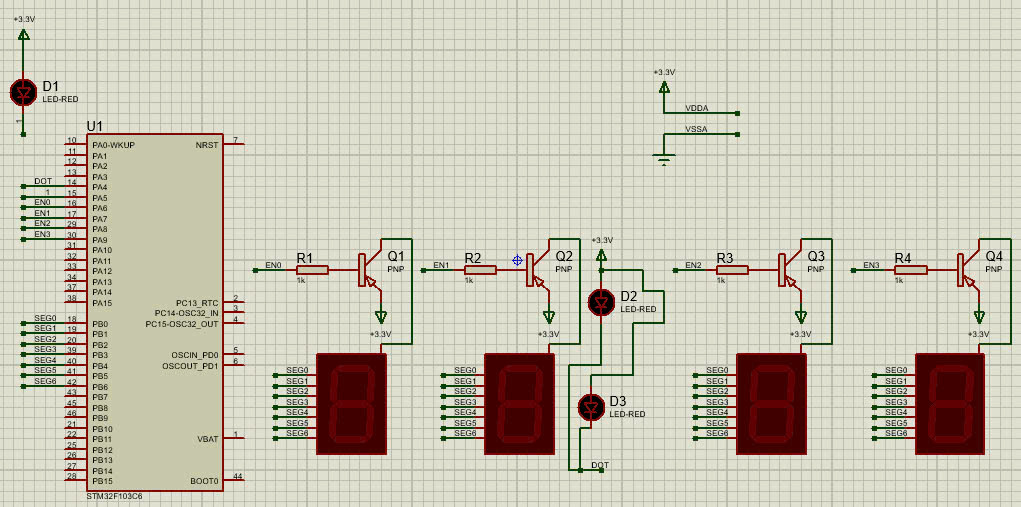
\includegraphics[width=5.5in]{source/picture/bai_2/pic2.jpg}
    \caption{\textit{ Schematic in Proteus}}
    \label{bai2_pic1a}
\end{figure}
\begin{lstlisting}[caption=main.c]
/* USER CODE BEGIN 2 */
  HAL_TIM_Base_Start_IT (& htim2 ) ;
  setTimer(0, 500);
  setTimer(1, 1000);
  /* USER CODE END 2 */

  /* Infinite loop */
  /* USER CODE BEGIN WHILE */
  while (1)
  {
	  if(isTimerExpired(0)==1){
	 		  setTimer(0, 500);
	 		  Ex2_run();
	 	  }
	  if(isTimerExpired(1)==1){
 		  setTimer(1, 1000);
 		  led_blinky();
 	  }
    /* USER CODE END WHILE */

    /* USER CODE BEGIN 3 */
  }
\end{lstlisting}
\begin{lstlisting}[caption=software$\_$timer2.c]
#include "software_timer2.h"

#define MAX_COUNTER 10
#define TIMER_TICK 10

int timer_counter[MAX_COUNTER];
int timer_flag[MAX_COUNTER];
int index_led=0;
int counter=0;

void display7SEG(int num) {
      const uint8_t segmentMap[10] = {
          0b11111100,
          0b01100000,
          0b11011010,
          0b11110010,
          0b01100110,
          0b10110110,
          0b10111110,
          0b11100000,
          0b11111110,
          0b11110110
      };
      HAL_GPIO_WritePin(SEG0_GPIO_Port, SEG0_Pin, (segmentMap[num] & 0b10000000) ? GPIO_PIN_RESET : GPIO_PIN_SET);
      HAL_GPIO_WritePin(SEG1_GPIO_Port, SEG1_Pin, (segmentMap[num] & 0b01000000) ? GPIO_PIN_RESET : GPIO_PIN_SET);
      HAL_GPIO_WritePin(SEG2_GPIO_Port, SEG2_Pin, (segmentMap[num] & 0b00100000) ? GPIO_PIN_RESET : GPIO_PIN_SET);
      HAL_GPIO_WritePin(SEG3_GPIO_Port, SEG3_Pin, (segmentMap[num] & 0b00010000) ? GPIO_PIN_RESET : GPIO_PIN_SET);
      HAL_GPIO_WritePin(SEG4_GPIO_Port, SEG4_Pin, (segmentMap[num] & 0b00001000) ? GPIO_PIN_RESET : GPIO_PIN_SET);
      HAL_GPIO_WritePin(SEG5_GPIO_Port, SEG5_Pin, (segmentMap[num] & 0b00000100) ? GPIO_PIN_RESET : GPIO_PIN_SET);
      HAL_GPIO_WritePin(SEG6_GPIO_Port, SEG6_Pin, (segmentMap[num] & 0b00000010) ? GPIO_PIN_RESET : GPIO_PIN_SET);
  }
  
void Ex2_run(){
	if(index_led>=4) index_led=0;
	index_led++;
	if(index_led<=1){
			HAL_GPIO_WritePin(EN1_GPIO_Port, EN1_Pin, SET);
			HAL_GPIO_WritePin(EN2_GPIO_Port, EN2_Pin, SET);
			HAL_GPIO_WritePin(EN3_GPIO_Port, EN3_Pin, SET);
			HAL_GPIO_WritePin(EN0_GPIO_Port, EN0_Pin, RESET);
			display7SEG(1);
	}
	if(index_led>=2&&index_led<3){
			HAL_GPIO_WritePin(EN0_GPIO_Port, EN0_Pin, SET);
			HAL_GPIO_WritePin(EN2_GPIO_Port, EN2_Pin, SET);
			HAL_GPIO_WritePin(EN3_GPIO_Port, EN3_Pin, SET);
			HAL_GPIO_WritePin(EN1_GPIO_Port, EN1_Pin, RESET);
		    display7SEG(2);
	}
	if(index_led>=3&&index_led<4){
			HAL_GPIO_WritePin(EN0_GPIO_Port, EN0_Pin, SET);
			HAL_GPIO_WritePin(EN1_GPIO_Port, EN1_Pin, SET);
			HAL_GPIO_WritePin(EN3_GPIO_Port, EN3_Pin, SET);
			HAL_GPIO_WritePin(EN2_GPIO_Port, EN2_Pin, RESET);
			display7SEG(3);
		}
	if(index_led>=4){
			HAL_GPIO_WritePin(EN0_GPIO_Port, EN0_Pin, SET);
			HAL_GPIO_WritePin(EN1_GPIO_Port, EN1_Pin, SET);
			HAL_GPIO_WritePin(EN2_GPIO_Port, EN2_Pin, SET);
			HAL_GPIO_WritePin(EN3_GPIO_Port, EN3_Pin, RESET);
			display7SEG(0);
		}
}

void led_blinky(){
	if(counter>=2) counter=0;
	counter++;
	if(counter<=1) HAL_GPIO_WritePin(DOT_GPIO_Port,DOT_Pin , RESET);
	else HAL_GPIO_WritePin(DOT_GPIO_Port,DOT_Pin , SET);
}

void setTimer(int index, int value){
	timer_counter[index]=value/TIMER_TICK;
	timer_flag[index]=0;
}

int isTimerExpired(int index){
	if(timer_flag[index]==1){
		timer_flag[index]=0;
		return 1;
	}
	return 0;
}

void timerRun(){
	for(int i=0;i<MAX_COUNTER;i++){
		if(timer_counter[i]>0){
			timer_counter[i]--;
			if(timer_counter[i]<=0) timer_flag[i]=1;
		}
	}
}
\end{lstlisting}
Short question: Tần số của quá trình quét là $\dfrac{1}{4\times0.5}$ = 0.5 Hz.
\subsection{Exercise 3, 8}
\begin{figure}[!htp]
    \centering
    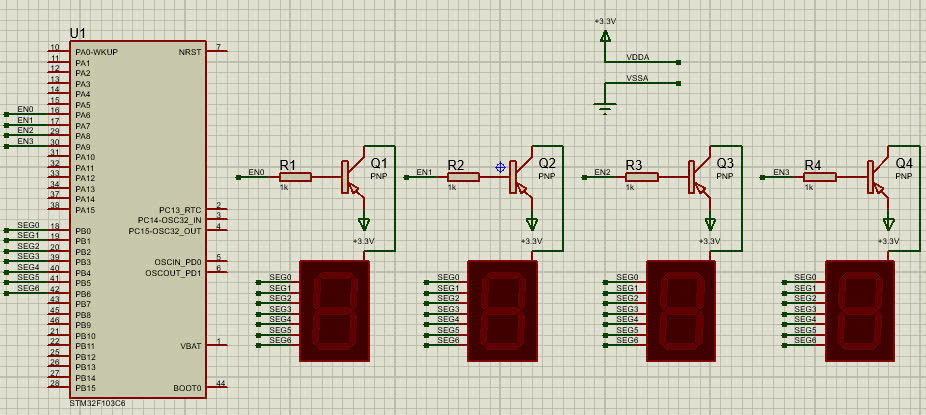
\includegraphics[width=5.5in]{source/picture/bai_2/pic3.jpg}
    \caption{\textit{ Schematic in Proteus}}
    \label{bai2_pic1a}
\end{figure}
\begin{lstlisting}[caption=main.c]
/* USER CODE BEGIN 2 */
  HAL_TIM_Base_Start_IT (& htim2 ) ;
  setTimer(0, 500);
  /* USER CODE END 2 */

  /* Infinite loop */
  /* USER CODE BEGIN WHILE */
  while (1)
  {
	  if(isTimerExpired(0)==1){
	  	 	setTimer(0, 500);
	  	 	Ex3_run();
	  }
    /* USER CODE END WHILE */

    /* USER CODE BEGIN 3 */
  }
\end{lstlisting}
\begin{lstlisting}[caption=software$\_$timer3.c]
#include "software_timer3.h"

#define MAX_COUNTER 10
#define TIMER_TICK 10

int timer_counter[MAX_COUNTER];
int timer_flag[MAX_COUNTER];
const int MAX_LED = 4;
int index_led = 0;
int led_buffer [4] = {1 , 2 , 3 , 4};

void display7SEG(int num) {
       const uint8_t segmentMap[10] = {
           0b11111100,
           0b01100000,
           0b11011010,
           0b11110010,
           0b01100110,
           0b10110110,
           0b10111110,
           0b11100000,
           0b11111110,
           0b11110110
       };
       HAL_GPIO_WritePin(SEG0_GPIO_Port, SEG0_Pin, (segmentMap[num] & 0b10000000) ? GPIO_PIN_RESET : GPIO_PIN_SET);
       HAL_GPIO_WritePin(SEG1_GPIO_Port, SEG1_Pin, (segmentMap[num] & 0b01000000) ? GPIO_PIN_RESET : GPIO_PIN_SET);
       HAL_GPIO_WritePin(SEG2_GPIO_Port, SEG2_Pin, (segmentMap[num] & 0b00100000) ? GPIO_PIN_RESET : GPIO_PIN_SET);
       HAL_GPIO_WritePin(SEG3_GPIO_Port, SEG3_Pin, (segmentMap[num] & 0b00010000) ? GPIO_PIN_RESET : GPIO_PIN_SET);
       HAL_GPIO_WritePin(SEG4_GPIO_Port, SEG4_Pin, (segmentMap[num] & 0b00001000) ? GPIO_PIN_RESET : GPIO_PIN_SET);
       HAL_GPIO_WritePin(SEG5_GPIO_Port, SEG5_Pin, (segmentMap[num] & 0b00000100) ? GPIO_PIN_RESET : GPIO_PIN_SET);
       HAL_GPIO_WritePin(SEG6_GPIO_Port, SEG6_Pin, (segmentMap[num] & 0b00000010) ? GPIO_PIN_RESET : GPIO_PIN_SET);
   }
   
void update7SEG ( int index ) {
	 switch ( index ) {
	 case 0:
	 // Display the first 7 SEG with led_buffer [0]
		 HAL_GPIO_WritePin(EN1_GPIO_Port, EN1_Pin, SET);
		 HAL_GPIO_WritePin(EN2_GPIO_Port, EN2_Pin, SET);
		 HAL_GPIO_WritePin(EN3_GPIO_Port, EN3_Pin, SET);
		 HAL_GPIO_WritePin(EN0_GPIO_Port, EN0_Pin, RESET);
		 display7SEG(led_buffer[index]);
	 break ;
	 case 1:
	 // Display the second 7 SEG with led_buffer [1]
		 HAL_GPIO_WritePin(EN0_GPIO_Port, EN0_Pin, SET);
		 HAL_GPIO_WritePin(EN2_GPIO_Port, EN2_Pin, SET);
		 HAL_GPIO_WritePin(EN3_GPIO_Port, EN3_Pin, SET);
		 HAL_GPIO_WritePin(EN1_GPIO_Port, EN1_Pin, RESET);
		 display7SEG(led_buffer[index]);
	 break ;
	 case 2:
	 // Display the third 7 SEG with led_buffer [2]
		 HAL_GPIO_WritePin(EN1_GPIO_Port, EN1_Pin, SET);
		 HAL_GPIO_WritePin(EN0_GPIO_Port, EN0_Pin, SET);
		 HAL_GPIO_WritePin(EN3_GPIO_Port, EN3_Pin, SET);
		 HAL_GPIO_WritePin(EN2_GPIO_Port, EN2_Pin, RESET);
		 display7SEG(led_buffer[index]);
	 break ;
	 case 3:
	 // Display the forth 7 SEG with led_buffer [3]
		 HAL_GPIO_WritePin(EN1_GPIO_Port, EN1_Pin, SET);
		 HAL_GPIO_WritePin(EN2_GPIO_Port, EN2_Pin, SET);
		 HAL_GPIO_WritePin(EN0_GPIO_Port, EN0_Pin, SET);
		 HAL_GPIO_WritePin(EN3_GPIO_Port, EN3_Pin, RESET);
		 display7SEG(led_buffer[index]);
	 break ;
	 default :
		 HAL_GPIO_WritePin(EN1_GPIO_Port, EN1_Pin, SET);
		 HAL_GPIO_WritePin(EN2_GPIO_Port, EN2_Pin, SET);
		 HAL_GPIO_WritePin(EN3_GPIO_Port, EN3_Pin, SET);
		 HAL_GPIO_WritePin(EN0_GPIO_Port, EN0_Pin, SET);
	 break ;
	 }
 }
 
void Ex3_run(){
	if(index_led>=MAX_LED) index_led=0;
		update7SEG(index_led++);
}

void setTimer(int index, int value){
	timer_counter[index]=value/TIMER_TICK;
	timer_flag[index]=0;
}

int isTimerExpired(int index){
	if(timer_flag[index]==1){
		timer_flag[index]=0;
		return 1;
	}
	return 0;
}

void timerRun(){
	for(int i=0;i<MAX_COUNTER;i++){
		if(timer_counter[i]>0){
			timer_counter[i]--;
			if(timer_counter[i]<=0) timer_flag[i]=1;
		}
	}
}
\end{lstlisting}
\subsection{Exercise 4}
\begin{figure}[!htp]
    \centering
    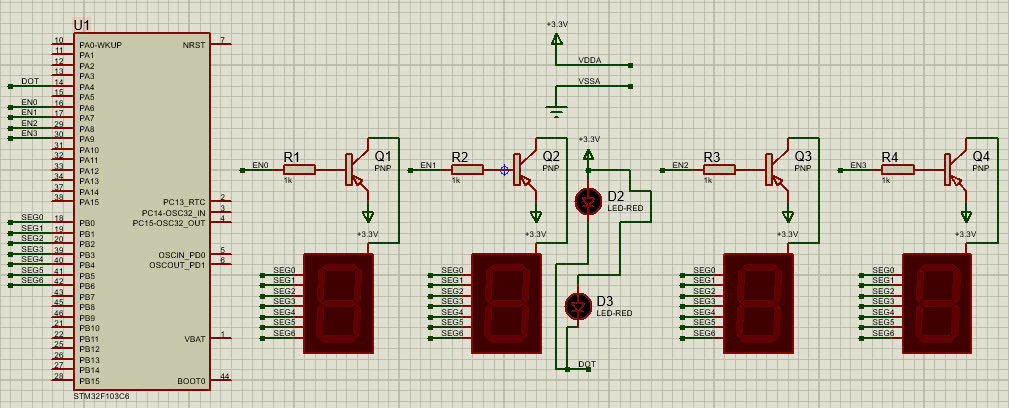
\includegraphics[width=5.5in]{source/picture/bai_2/pic4.jpg}
    \caption{\textit{ Schematic in Proteus}}
    \label{bai2_pic1a}
\end{figure}
\begin{lstlisting}[caption=main.c]
/* USER CODE BEGIN 2 */
  HAL_TIM_Base_Start_IT (& htim2 ) ;
  setTimer(0, 250);
  setTimer(1, 1000);
  /* USER CODE END 2 */

  /* Infinite loop */
  /* USER CODE BEGIN WHILE */
  while (1)
  {
	  if(isTimerExpired(0)==1){
	 	  	setTimer(0, 250);
	 	  	Ex4_run();
	 }
	  if(isTimerExpired(1)==1){
	 	  	setTimer(1, 1000);
	 	  	led_blinky();
	 }
    /* USER CODE END WHILE */

    /* USER CODE BEGIN 3 */
  }
\end{lstlisting}
\begin{lstlisting}[caption=software$\_$timer4.c]
#include "software_timer4.h"

#define MAX_COUNTER 10
#define TIMER_TICK 10

int timer_counter[MAX_COUNTER];
int timer_flag[MAX_COUNTER];
int counter=0;
const int MAX_LED = 4;
int index_led = 0;
int led_buffer [4] = {1 , 2 , 3 , 4};

void display7SEG(int num) {
       const uint8_t segmentMap[10] = {
           0b11111100,
           0b01100000,
           0b11011010,
           0b11110010,
           0b01100110,
           0b10110110,
           0b10111110,
           0b11100000,
           0b11111110,
           0b11110110
       };
       HAL_GPIO_WritePin(SEG0_GPIO_Port, SEG0_Pin, (segmentMap[num] & 0b10000000) ? GPIO_PIN_RESET : GPIO_PIN_SET);
       HAL_GPIO_WritePin(SEG1_GPIO_Port, SEG1_Pin, (segmentMap[num] & 0b01000000) ? GPIO_PIN_RESET : GPIO_PIN_SET);
       HAL_GPIO_WritePin(SEG2_GPIO_Port, SEG2_Pin, (segmentMap[num] & 0b00100000) ? GPIO_PIN_RESET : GPIO_PIN_SET);
       HAL_GPIO_WritePin(SEG3_GPIO_Port, SEG3_Pin, (segmentMap[num] & 0b00010000) ? GPIO_PIN_RESET : GPIO_PIN_SET);
       HAL_GPIO_WritePin(SEG4_GPIO_Port, SEG4_Pin, (segmentMap[num] & 0b00001000) ? GPIO_PIN_RESET : GPIO_PIN_SET);
       HAL_GPIO_WritePin(SEG5_GPIO_Port, SEG5_Pin, (segmentMap[num] & 0b00000100) ? GPIO_PIN_RESET : GPIO_PIN_SET);
       HAL_GPIO_WritePin(SEG6_GPIO_Port, SEG6_Pin, (segmentMap[num] & 0b00000010) ? GPIO_PIN_RESET : GPIO_PIN_SET);
   }
   
void update7SEG ( int index ) {
	 switch ( index ) {
	 case 0:
	 // Display the first 7 SEG with led_buffer [0]
		 HAL_GPIO_WritePin(EN1_GPIO_Port, EN1_Pin, SET);
		 HAL_GPIO_WritePin(EN2_GPIO_Port, EN2_Pin, SET);
		 HAL_GPIO_WritePin(EN3_GPIO_Port, EN3_Pin, SET);
		 HAL_GPIO_WritePin(EN0_GPIO_Port, EN0_Pin, RESET);
		 display7SEG(led_buffer[index]);
	 break ;
	 case 1:
	 // Display the second 7 SEG with led_buffer [1]
		 HAL_GPIO_WritePin(EN0_GPIO_Port, EN0_Pin, SET);
		 HAL_GPIO_WritePin(EN2_GPIO_Port, EN2_Pin, SET);
		 HAL_GPIO_WritePin(EN3_GPIO_Port, EN3_Pin, SET);
		 HAL_GPIO_WritePin(EN1_GPIO_Port, EN1_Pin, RESET);
		 display7SEG(led_buffer[index]);
	 break ;
	 case 2:
	 // Display the third 7 SEG with led_buffer [2]
		 HAL_GPIO_WritePin(EN1_GPIO_Port, EN1_Pin, SET);
		 HAL_GPIO_WritePin(EN0_GPIO_Port, EN0_Pin, SET);
		 HAL_GPIO_WritePin(EN3_GPIO_Port, EN3_Pin, SET);
		 HAL_GPIO_WritePin(EN2_GPIO_Port, EN2_Pin, RESET);
		 display7SEG(led_buffer[index]);
	 break ;
	 case 3:
	 // Display the forth 7 SEG with led_buffer [3]
		 HAL_GPIO_WritePin(EN1_GPIO_Port, EN1_Pin, SET);
		 HAL_GPIO_WritePin(EN2_GPIO_Port, EN2_Pin, SET);
		 HAL_GPIO_WritePin(EN0_GPIO_Port, EN0_Pin, SET);
		 HAL_GPIO_WritePin(EN3_GPIO_Port, EN3_Pin, RESET);
		 display7SEG(led_buffer[index]);
	 break ;
	 default :
		 HAL_GPIO_WritePin(EN1_GPIO_Port, EN1_Pin, SET);
		 HAL_GPIO_WritePin(EN2_GPIO_Port, EN2_Pin, SET);
		 HAL_GPIO_WritePin(EN3_GPIO_Port, EN3_Pin, SET);
		 HAL_GPIO_WritePin(EN0_GPIO_Port, EN0_Pin, SET);
	 break ;
	 }
 }
 
void led_blinky(){
 	if(counter>=2) counter=0;
 	counter++;
 	if(counter<=1) HAL_GPIO_WritePin(DOT_GPIO_Port,DOT_Pin , RESET);
 	else HAL_GPIO_WritePin(DOT_GPIO_Port,DOT_Pin , SET);
 }
 
void Ex4_run(){
	if(index_led>=MAX_LED) index_led=0;
		update7SEG(index_led++);
}

void setTimer(int index, int value){
	timer_counter[index]=value/TIMER_TICK;
	timer_flag[index]=0;
}

int isTimerExpired(int index){
	if(timer_flag[index]==1){
		timer_flag[index]=0;
		return 1;
	}
	return 0;
}

void timerRun(){
	for(int i=0;i<MAX_COUNTER;i++){
		if(timer_counter[i]>0){
			timer_counter[i]--;
			if(timer_counter[i]<=0) timer_flag[i]=1;
		}
	}
}
\end{lstlisting}
\newpage
\subsection{Exercise 5, 7}
\begin{figure}[!htp]
    \centering
    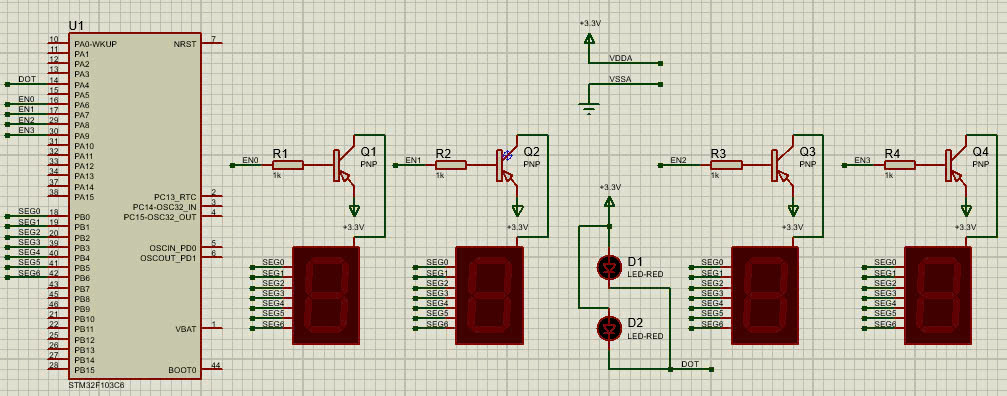
\includegraphics[width=5.5in]{source/picture/bai_2/pic5.jpg}
    \caption{\textit{ Schematic in Proteus}}
    \label{bai2_pic1a}
\end{figure}

\begin{lstlisting}[caption=main.c]
/* USER CODE BEGIN 2 */
  HAL_TIM_Base_Start_IT (& htim2 ) ;
    setTimer(0, 250);
    setTimer(1, 1000);
    setTimer(2, 1000);
  /* USER CODE END 2 */

  /* Infinite loop */
  /* USER CODE BEGIN WHILE */
  while (1)
  {
	  if(isTimerExpired(0)==1){
	  	 	  	setTimer(0, 250);
	  	 	  	scan_7LED();
	  	 }
	  	if(isTimerExpired(1)==1){
	  		  	setTimer(1, 1000);
	  		  	Ex5_run();
	  	}
	  	if(isTimerExpired(2)==1){
	  		  	setTimer(2, 1000);
	  		  	led_blinky();
	  	}

    /* USER CODE END WHILE */

    /* USER CODE BEGIN 3 */
  }
\end{lstlisting}
\begin{lstlisting}[caption=software$\_$timer5.c]
#include "software_timer5.h"
#define MAX_COUNTER 10
#define TIMER_TICK 10

int timer_counter[MAX_COUNTER];
int timer_flag[MAX_COUNTER];

int hour = 15 , minute = 8 , second = 50;
int counter=0;
const int MAX_LED = 4;
 int index_led = 0;
 int led_buffer [4] = {1 , 5 , 0 , 8};

 void updateClockBuffer (){
 	led_buffer[0]=hour/10;
 	led_buffer[1]=hour%10;
 	led_buffer[2]=minute/10;
 	led_buffer[3]=minute%10;
 }
 void Ex5_run(){
 	second ++;
 	 if ( second >= 60) {
 		 second = 0;
 		 minute ++;
 	}
 	if( minute >= 60) {
 		 minute = 0;
 		 hour ++;
 	}
 	if( hour >=24) {
 		 hour = 0;
 	}
 	updateClockBuffer();
 }

 void display7SEG(int num) {
       const uint8_t segmentMap[10] = {
    		   	  0b11111100, // 0
    		      0b01100000, // 1
    		      0b11011010, // 2
    		      0b11110010, // 3
    		      0b01100110, // 4
    		      0b10110110, // 5
    		      0b10111110, // 6
    		      0b11100000, // 7
    		      0b11111110, // 8
    		      0b11110110  // 9
       };
       HAL_GPIO_WritePin(SEG0_GPIO_Port, SEG0_Pin, (segmentMap[num] & 0b10000000) ? GPIO_PIN_RESET : GPIO_PIN_SET);
       HAL_GPIO_WritePin(SEG1_GPIO_Port, SEG1_Pin, (segmentMap[num] & 0b01000000) ? GPIO_PIN_RESET : GPIO_PIN_SET);
       HAL_GPIO_WritePin(SEG2_GPIO_Port, SEG2_Pin, (segmentMap[num] & 0b00100000) ? GPIO_PIN_RESET : GPIO_PIN_SET);
       HAL_GPIO_WritePin(SEG3_GPIO_Port, SEG3_Pin, (segmentMap[num] & 0b00010000) ? GPIO_PIN_RESET : GPIO_PIN_SET);
       HAL_GPIO_WritePin(SEG4_GPIO_Port, SEG4_Pin, (segmentMap[num] & 0b00001000) ? GPIO_PIN_RESET : GPIO_PIN_SET);
       HAL_GPIO_WritePin(SEG5_GPIO_Port, SEG5_Pin, (segmentMap[num] & 0b00000100) ? GPIO_PIN_RESET : GPIO_PIN_SET);
       HAL_GPIO_WritePin(SEG6_GPIO_Port, SEG6_Pin, (segmentMap[num] & 0b00000010) ? GPIO_PIN_RESET : GPIO_PIN_SET);
   }
 void update7SEG ( int index ) {
	 switch ( index ) {
	 case 0:
	 // Display the first 7 SEG with led_buffer [0]
		 HAL_GPIO_WritePin(EN1_GPIO_Port, EN1_Pin, SET);
		 HAL_GPIO_WritePin(EN2_GPIO_Port, EN2_Pin, SET);
		 HAL_GPIO_WritePin(EN3_GPIO_Port, EN3_Pin, SET);
		 HAL_GPIO_WritePin(EN0_GPIO_Port, EN0_Pin, RESET);
		 display7SEG(led_buffer[index]);
	 break ;
	 case 1:
	 // Display the second 7 SEG with led_buffer [1]
		 HAL_GPIO_WritePin(EN0_GPIO_Port, EN0_Pin, SET);
		 HAL_GPIO_WritePin(EN2_GPIO_Port, EN2_Pin, SET);
		 HAL_GPIO_WritePin(EN3_GPIO_Port, EN3_Pin, SET);
		 HAL_GPIO_WritePin(EN1_GPIO_Port, EN1_Pin, RESET);
		 display7SEG(led_buffer[index]);
	 break ;
	 case 2:
	 // Display the third 7 SEG with led_buffer [2]
		 HAL_GPIO_WritePin(EN1_GPIO_Port, EN1_Pin, SET);
		 HAL_GPIO_WritePin(EN0_GPIO_Port, EN0_Pin, SET);
		 HAL_GPIO_WritePin(EN3_GPIO_Port, EN3_Pin, SET);
		 HAL_GPIO_WritePin(EN2_GPIO_Port, EN2_Pin, RESET);
		 display7SEG(led_buffer[index]);
	 break ;
	 case 3:
	 // Display the forth 7 SEG with led_buffer [3]
		 HAL_GPIO_WritePin(EN1_GPIO_Port, EN1_Pin, SET);
		 HAL_GPIO_WritePin(EN2_GPIO_Port, EN2_Pin, SET);
		 HAL_GPIO_WritePin(EN0_GPIO_Port, EN0_Pin, SET);
		 HAL_GPIO_WritePin(EN3_GPIO_Port, EN3_Pin, RESET);
		 display7SEG(led_buffer[index]);
	 break ;
	 default :
		 HAL_GPIO_WritePin(EN1_GPIO_Port, EN1_Pin, SET);
		 HAL_GPIO_WritePin(EN2_GPIO_Port, EN2_Pin, SET);
		 HAL_GPIO_WritePin(EN3_GPIO_Port, EN3_Pin, SET);
		 HAL_GPIO_WritePin(EN0_GPIO_Port, EN0_Pin, SET);
	 break ;
	 }
 }
 void led_blinky(){
 	if(counter>=2) counter=0;
 	counter++;
 	if(counter<=1) HAL_GPIO_WritePin(DOT_GPIO_Port,DOT_Pin , RESET);
 	else HAL_GPIO_WritePin(DOT_GPIO_Port,DOT_Pin , SET);
 }
void scan_7LED(){
	if(index_led>=MAX_LED) {
		index_led=0;
	}
		update7SEG(index_led++);
}


void setTimer(int index, int value){
	timer_counter[index]=value/TIMER_TICK;
	timer_flag[index]=0;
}

int isTimerExpired(int index){
	if(timer_flag[index]==1){
		timer_flag[index]=0;
		return 1;
	}
	return 0;
}

void timerRun(){
	for(int i=0;i<MAX_COUNTER;i++){
		if(timer_counter[i]>0){
			timer_counter[i]--;
			if(timer_counter[i]<=0) timer_flag[i]=1;
		}
	}
}
\end{lstlisting}


\subsection{Exercise 6}
Nếu dòng 1 của đoạn mã trên bị miss thì chỉ còn 99 lần gọi hàm ngắt mỗi 10 ms do lần đầu chạy quá nhanh nó xảy ra ngắt liền, sai số về thời gian lúc này chỉ là $\dfrac{1}{100}$ = 1$\%$.\\
Nếu dòng 1 của đoạn mã trên bị thay đổi thành setTimer0(1), thì vòng lặp while không gọi hàm ngắt mỗi 10 ms được vì sai số về thời gian lúc này lên đến là $\dfrac{1}{0.1}$ = 1000$\%$.\\
Nếu dòng 1 của đoạn mã trên bị thay đổi thành setTimer0(10), thì vòng lặp while không gọi hàm ngắt mỗi 10 ms được vì sai số về thời gian lúc này lên đến là $\dfrac{1}{1}$ = 100$\%$ dẫn đến đèn led không chớp tắt được.


\subsection{Exercise 9}
\begin{figure}[!htp]
    \centering
    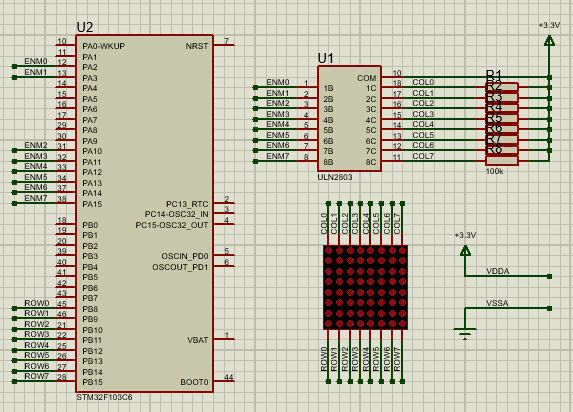
\includegraphics[width=5.5in]{source/picture/bai_2/pic9.jpg}
    \caption{\textit{LED matrix is added to the simulation}}
    \label{bai2_pic9}
\end{figure}



\begin{lstlisting}[caption=main.c]
/* USER CODE BEGIN 2 */
  HAL_TIM_Base_Start_IT (& htim2 ) ;
  setTimer(0, 10);
  /* USER CODE END 2 */

  /* Infinite loop */
  /* USER CODE BEGIN WHILE */
  while (1)
  {
	  if(isTimerExpired(0)==1){
		  setTimer(0, 10);
		  Ex9_run();
	  }
    /* USER CODE END WHILE */

    /* USER CODE BEGIN 3 */
  }
\end{lstlisting}
\begin{lstlisting}[caption=software$\_$timer9.c]
#include "software_timer9.h"

#define MAX_COUNTER 10
#define TIMER_TICK 10

int timer_counter[MAX_COUNTER];
int timer_flag[MAX_COUNTER];
const int MAX_LED_MATRIX = 8;
int index_led_matrix = 0;
uint8_t matrix_buffer [8] = {0xFF , 0xC0 , 0x80 , 0x33 , 0x33 , 0x80 , 0xC0 , 0xFF };
uint16_t segmentPins[8] = {ROW0_Pin,ROW1_Pin,ROW2_Pin,ROW3_Pin,ROW4_Pin,ROW5_Pin,ROW6_Pin,ROW7_Pin};

void displayMatrix(uint8_t num){
	 for(int i=0;i<MAX_LED_MATRIX;i++){
		 HAL_GPIO_WritePin(GPIOB, segmentPins[i], (num&(0x80>>i))?SET:RESET);
	 }
 }
 
void Ex9_run(){
	 if(index_led_matrix>=8) index_led_matrix=0;
	 updateLEDMatrix(index_led_matrix++);
 }
 
void updateLEDMatrix (int index ) {
	 HAL_GPIO_WritePin(GPIOA, LED_Pins, SET);
		 switch ( index ) {
		 case 0:
			 HAL_GPIO_WritePin(GPIOA, ENM0_Pin, RESET);
			 displayMatrix(matrix_buffer[index]);
		 break ;
		 case 1:
			 HAL_GPIO_WritePin(GPIOA, ENM1_Pin, RESET);
			 displayMatrix(matrix_buffer[index]);
		 break ;
		 case 2:
			 HAL_GPIO_WritePin(GPIOA, ENM2_Pin, RESET);
			 displayMatrix(matrix_buffer[index]);
		 break ;
		 case 3:
			 HAL_GPIO_WritePin(GPIOA, ENM3_Pin, RESET);
			 displayMatrix(matrix_buffer[index]);
		 break ;
		 case 4:
			 HAL_GPIO_WritePin(GPIOA, ENM4_Pin, RESET);
			 displayMatrix(matrix_buffer[index]);
		 break ;
		 case 5:
			 HAL_GPIO_WritePin(GPIOA, ENM5_Pin, RESET);
			 displayMatrix(matrix_buffer[index]);
		 break ;
		 case 6:
			 HAL_GPIO_WritePin(GPIOA, ENM6_Pin, RESET);
			 displayMatrix(matrix_buffer[index]);
		 break ;
		 case 7:
			 HAL_GPIO_WritePin(GPIOA, ENM7_Pin, RESET);
			 displayMatrix(matrix_buffer[index]);
		 break ;
		 default :
			 HAL_GPIO_WritePin(GPIOA, LED_Pins , SET);
		 break ;
	}
 }

void setTimer(int index, int value){
	timer_counter[index]=value/TIMER_TICK;
	timer_flag[index]=0;
}
int isTimerExpired(int index){
	if(timer_flag[index]==1){
		timer_flag[index]=0;
		return 1;
	}
	return 0;
}
void timerRun(){
	for(int i=0;i<MAX_COUNTER;i++){
		if(timer_counter[i]>0){
			timer_counter[i]--;
			if(timer_counter[i]<=0) timer_flag[i]=1;
		}
	}
}
\end{lstlisting}
\subsection{Exercise 10}
\begin{figure}[!htp]
    \centering
    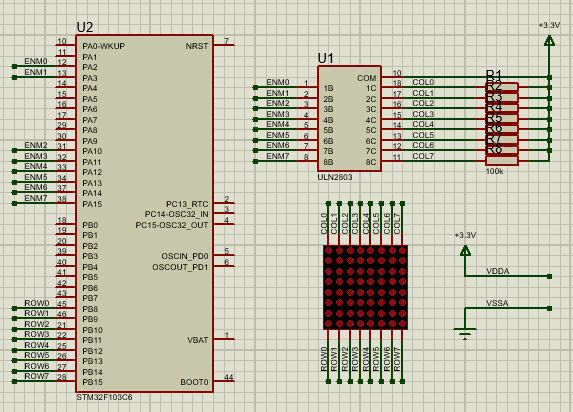
\includegraphics[width=5.5in]{source/picture/bai_2/pic9.jpg}
    \caption{\textit{LED matrix is added to the simulation}}
    \label{bai2_pic9}
\end{figure}
\begin{lstlisting}[caption=main.c]
/* USER CODE BEGIN 2 */
  HAL_TIM_Base_Start_IT (& htim2 ) ;
  setTimer(0, 10);
  setTimer(1, 80);
  /* USER CODE END 2 */

  /* Infinite loop */
  /* USER CODE BEGIN WHILE */
  while (1)
  {
	  if(isTimerExpired(0)==1){
		  setTimer(0, 10);
		  Ex10_run();
	  }
	  if(isTimerExpired(1)==1){
	  		setTimer(1, 80);
//	  		shiftColLeft();
//	  		shiftColRight();
//	  		shiftRowUp();
//	  		shiftRowDown();
	  	  }
    /* USER CODE END WHILE */

    /* USER CODE BEGIN 3 */
  }
\end{lstlisting}
\begin{lstlisting}[caption=software$\_$timer10.c]
#include "software_timer10.h"

#define MAX_COUNTER 10
#define TIMER_TICK 10

int timer_counter[MAX_COUNTER];
int timer_flag[MAX_COUNTER];
const int MAX_LED_MATRIX = 8;
int index_led_matrix = 0;
uint8_t matrix_buffer [8] = {0xFF , 0xC0 , 0x80 , 0x33 , 0x33 , 0x80 , 0xC0 , 0xFF };
uint16_t segmentPins[8] = {ROW0_Pin,ROW1_Pin,ROW2_Pin,ROW3_Pin,ROW4_Pin,ROW5_Pin,ROW6_Pin,ROW7_Pin};

void displayMatrix(uint8_t num){
	 for(int i=0;i<MAX_LED_MATRIX;i++){
		 HAL_GPIO_WritePin(GPIOB, segmentPins[i], (num&(0x80>>i))?SET:RESET);
	 }
 }
 
void shiftColLeft(){
	 for(int i=0;i<MAX_LED_MATRIX-1;i++){
		 matrix_buffer[i]=matrix_buffer[i+1];
	 }
	 matrix_buffer[7]=matrix_buffer[0];
 }
 
void shiftColRight(){
 	 for(int i=MAX_LED_MATRIX-1;i>0;i--){
 		 matrix_buffer[i]=matrix_buffer[i-1];
 	 }
 	 matrix_buffer[0]=matrix_buffer[7];
  }
  
void shiftRowUp(){
	 for (int i = 0; i < MAX_LED_MATRIX; i++) {
	         uint8_t temp = (matrix_buffer[i] & 0x80) ? 1 : 0;
	         matrix_buffer[i] <<= 1;
	         matrix_buffer[i] |= temp;
	     }
   }
   
void shiftRowDown(){
 	 for (int i = 0; i < MAX_LED_MATRIX; i++) {
 		uint8_t temp = (matrix_buffer[i] & 0x01) ? 0x80 : 0;
 	         matrix_buffer[i] >>= 1;
 	         matrix_buffer[i] |= temp;
 	     }
    }
    
void Ex10_run(){
	 if(index_led_matrix>=8) index_led_matrix=0;
	 updateLEDMatrix(index_led_matrix++);
 }
 
void updateLEDMatrix (int index ) {
	 HAL_GPIO_WritePin(GPIOA, LED_Pins, SET);
		 switch ( index ) {
		 case 0:
			 HAL_GPIO_WritePin(GPIOA, ENM0_Pin, RESET);
			 displayMatrix(matrix_buffer[index]);
		 break ;
		 case 1:
			 HAL_GPIO_WritePin(GPIOA, ENM1_Pin, RESET);
			 displayMatrix(matrix_buffer[index]);
		 break ;
		 case 2:
			 HAL_GPIO_WritePin(GPIOA, ENM2_Pin, RESET);
			 displayMatrix(matrix_buffer[index]);
		 break ;
		 case 3:
			 HAL_GPIO_WritePin(GPIOA, ENM3_Pin, RESET);
			 displayMatrix(matrix_buffer[index]);
		 break ;
		 case 4:
			 HAL_GPIO_WritePin(GPIOA, ENM4_Pin, RESET);
			 displayMatrix(matrix_buffer[index]);
		 break ;
		 case 5:
			 HAL_GPIO_WritePin(GPIOA, ENM5_Pin, RESET);
			 displayMatrix(matrix_buffer[index]);
		 break ;
		 case 6:
			 HAL_GPIO_WritePin(GPIOA, ENM6_Pin, RESET);
			 displayMatrix(matrix_buffer[index]);
		 break ;
		 case 7:
			 HAL_GPIO_WritePin(GPIOA, ENM7_Pin, RESET);
			 displayMatrix(matrix_buffer[index]);
		 break ;
		 default :
			 HAL_GPIO_WritePin(GPIOA, LED_Pins , SET);
		 break ;
	}
 }

void setTimer(int index, int value){
	timer_counter[index]=value/TIMER_TICK;
	timer_flag[index]=0;
}

int isTimerExpired(int index){
	if(timer_flag[index]==1){
		timer_flag[index]=0;
		return 1;
	}
	return 0;
}

void timerRun(){
	for(int i=0;i<MAX_COUNTER;i++){
		if(timer_counter[i]>0){
			timer_counter[i]--;
			if(timer_counter[i]<=0) timer_flag[i]=1;
		}
	}
}
\end{lstlisting}
Trong bài này các hàm trong vòng lặp while lần lượt dùng để dịch ký tự "A" sang trái, phải so với cột ma trận, dịch lên, xuống so với hàng ma trận, cứ mỗi lần tất cả các cột đều được quét qua thì lại cập nhập giá trị mới của mỗi cột và cứ lặp lại như thế .